\documentclass{lab}
\usepackage{subcaption} % For subfigure environment

\title{Lab \# 4. Detecting Human Gestures via Sound Signals} % Title

\author{Adan Abu Naaj | adann@mit.edu \\ Artem Laptiev | laptiev@mit.edu \\\\ 6.1820} % Team # + Names, Class (RSS)

\date{\today} % Date for the report

\begin{document}

\maketitle

\newpage

\section{Received FMCW Chirp}

The transmitted FMCW chirp is a linear frequency modulated signal that sweeps from a start frequency to an end frequency over a chirp time duration. Plotting the FFT of the original signal should theoretically show a square shape in the frequency domain, indicating the bandwidth of the chirp.

In contrast, the received FMCW chirp shows a shape of the same signal, distorted by the artifacts from the environment. 


\begin{figure}[h]
    \centering
    \begin{subfigure}[b]{0.48\textwidth}
        \centering
        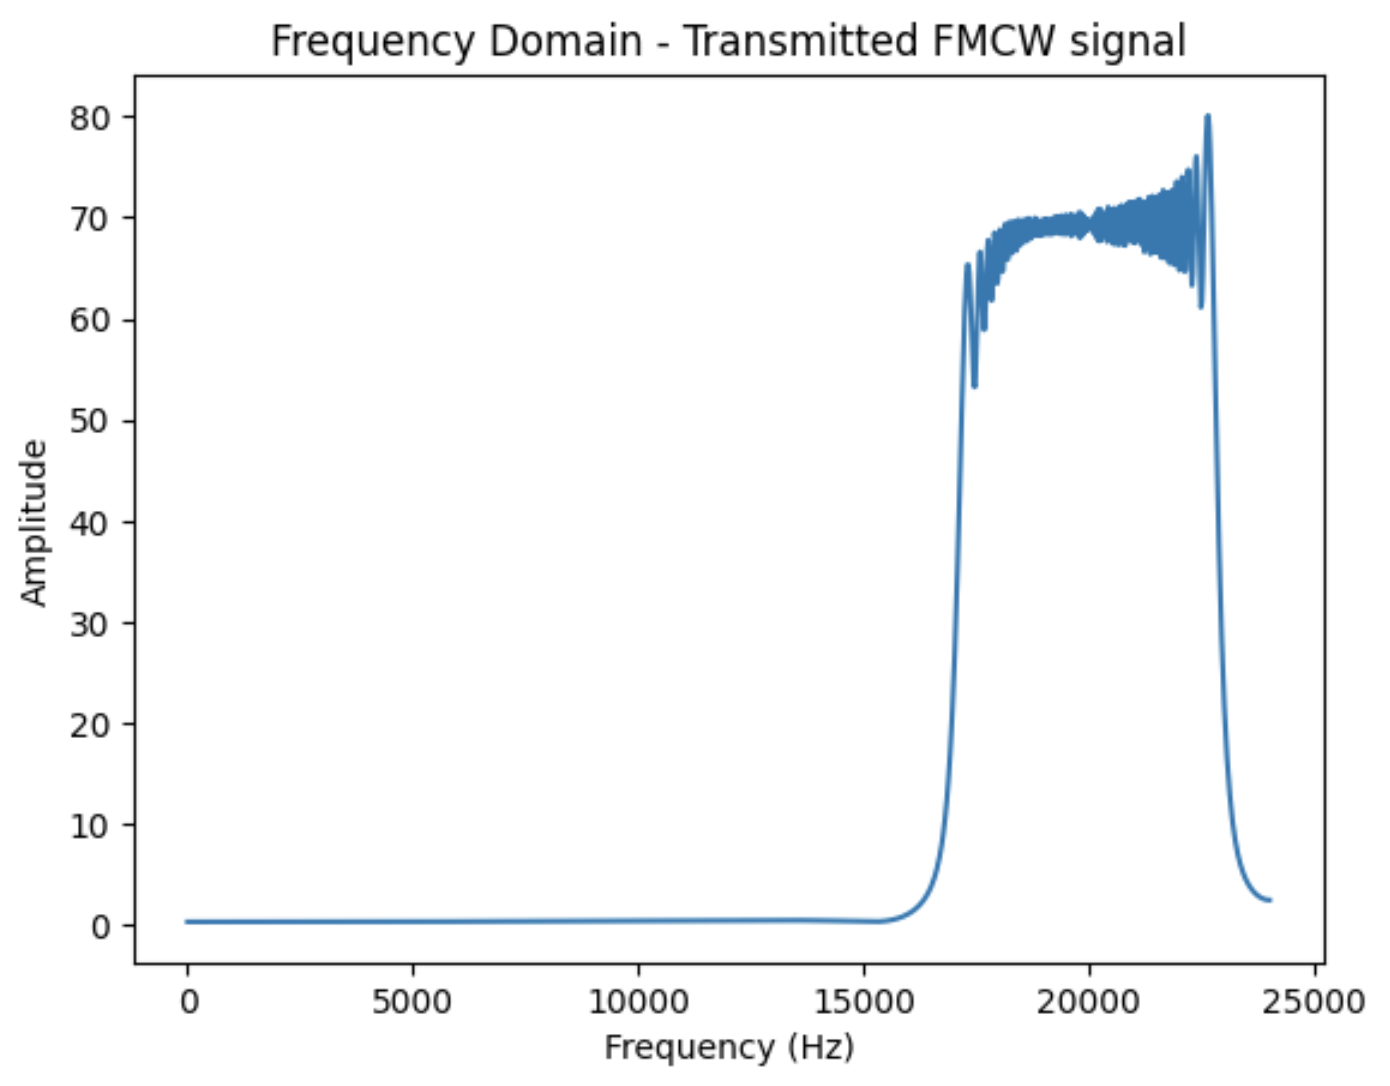
\includegraphics[width=\textwidth]{images/transmittedFMCW.png}
    \end{subfigure}
    \hfill
    \begin{subfigure}[b]{0.48\textwidth}
        \centering
        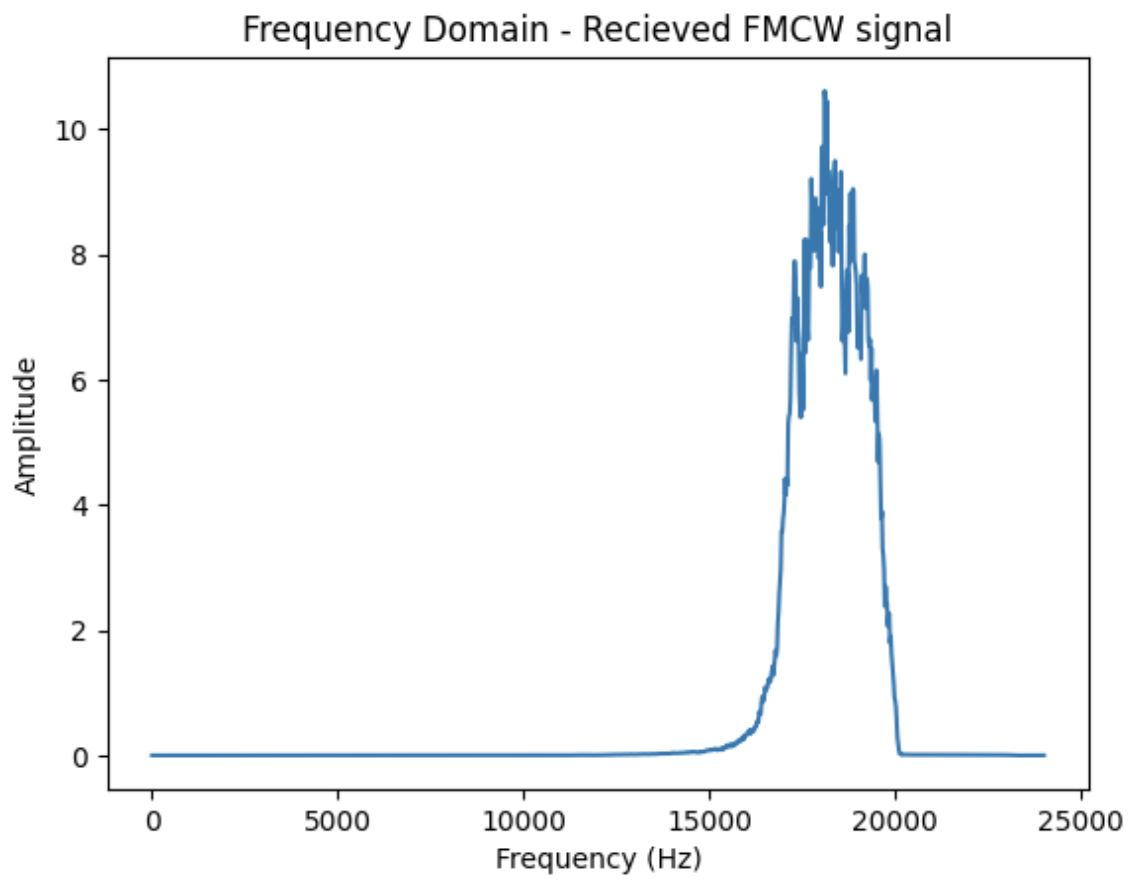
\includegraphics[width=\textwidth]{images/receivedFMCW.png}
    \end{subfigure}
    \caption{Comparison of transmitted and received FMCW chirp FFTs.}
\end{figure}


\section{Downconverted FMCW Chirp}

The downconverted FMCW chirp is the IF signal, a mix of the transmitted and received signals. The frequency of the IF signal corresponds to the difference in frequencies of the transmitted and received signals, which is depandand of the time delay (which in turn corresponds to the distance of the object). So, the FFT of the downconverted FMCW chirp shows a few high frequency peaks, indicating the presence of the object, and the high-frequency noise from the environment.

\begin{figure}[h]
    \begin{center}
    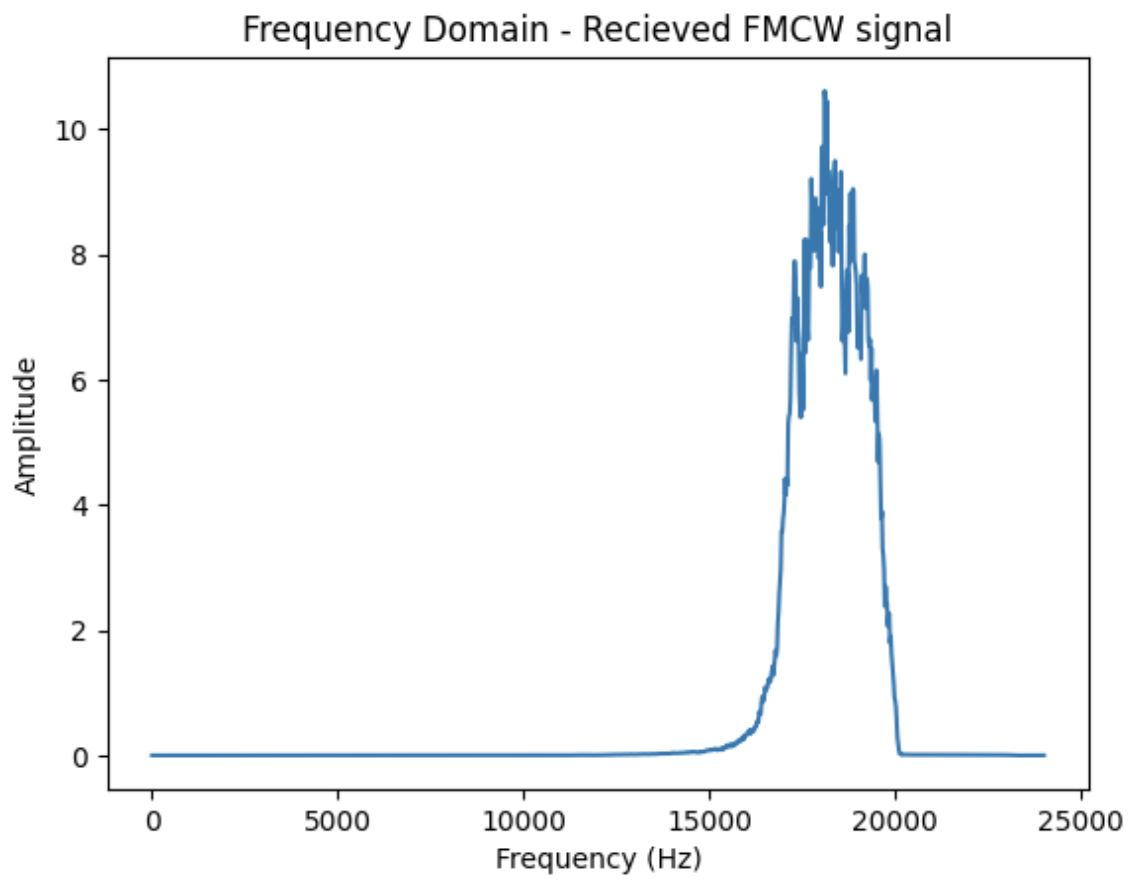
\includegraphics[width=0.65\textwidth]{images/receivedFMCW.png} 
    \caption{Downconverted FMCW chirp FFT.}
    \end{center}
\end{figure}

\pagebreak

\section{Experiments}

\begin{figure}[h]
    \centering
    \begin{subfigure}[b]{0.48\textwidth}
        \centering
        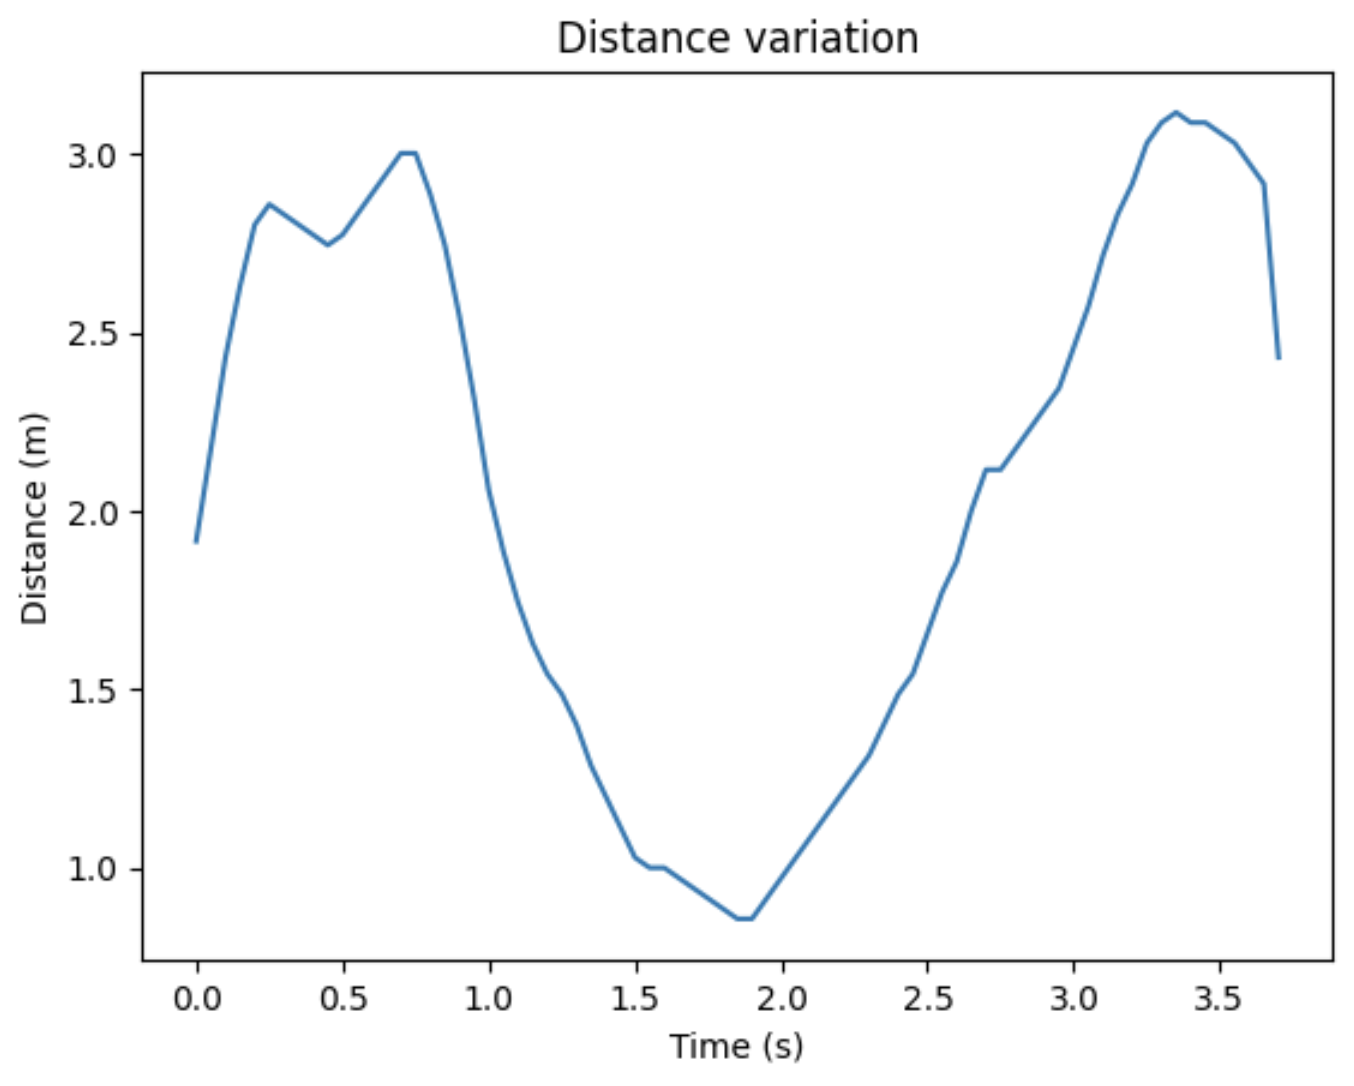
\includegraphics[width=\textwidth]{images/slow-time.png}
    \end{subfigure}
    \hfill
    \begin{subfigure}[b]{0.48\textwidth}
        \centering
        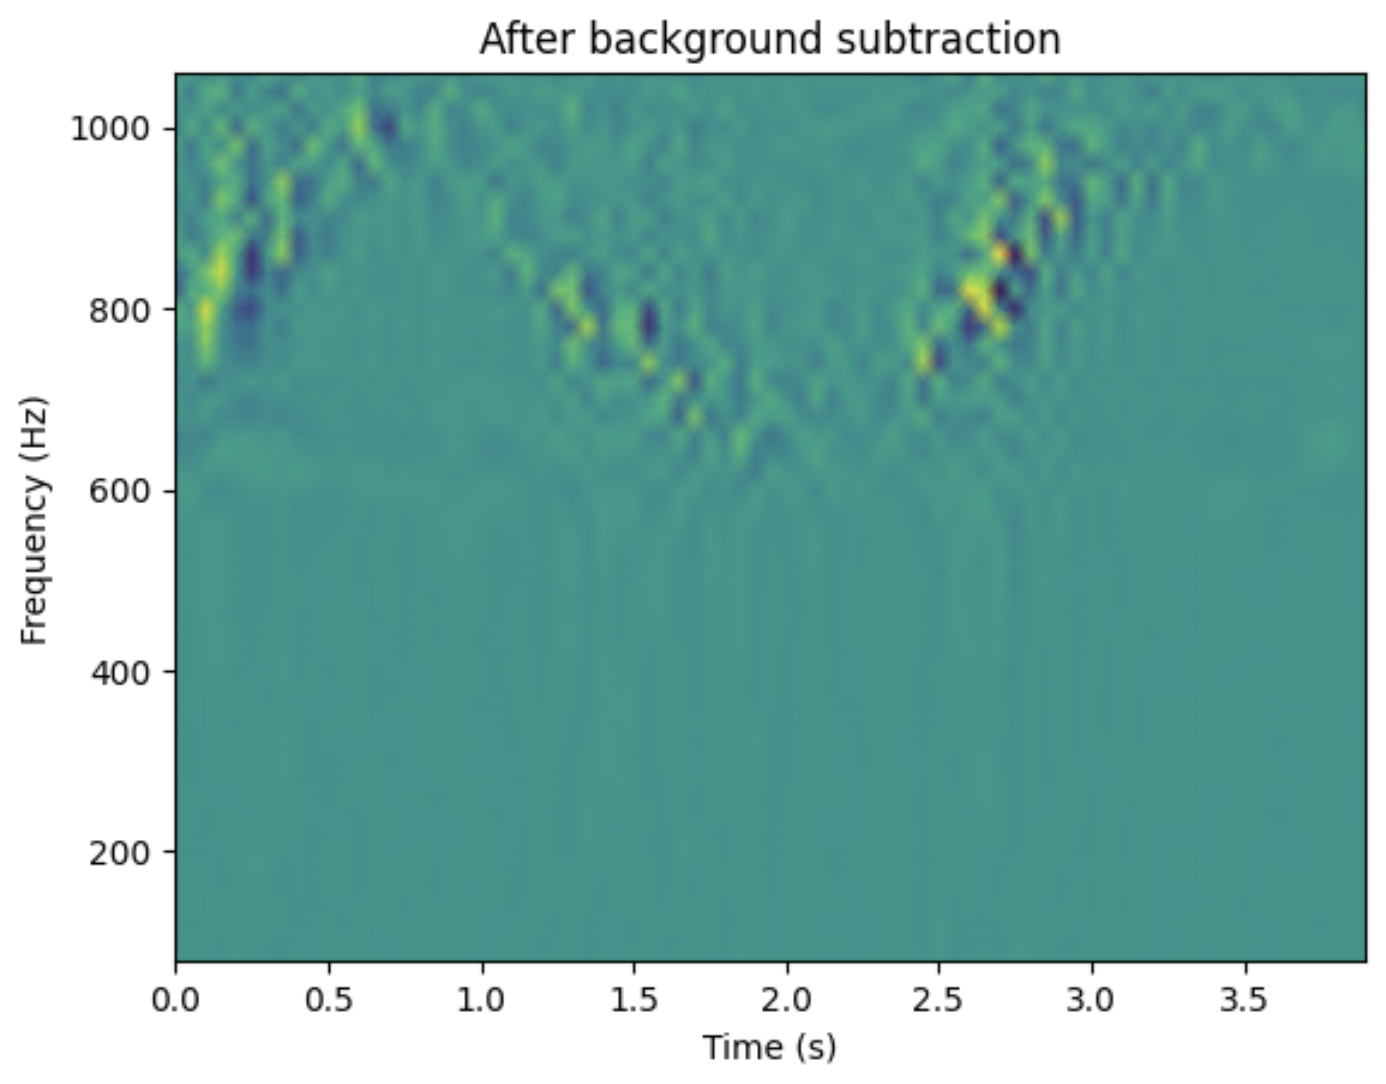
\includegraphics[width=\textwidth]{images/slow-freq.png}
    \end{subfigure}
    \caption{Slow experiment. Time and Frequency plots.}
\end{figure}


\begin{figure}[h]
    \centering
    \begin{subfigure}[b]{0.48\textwidth}
        \centering
        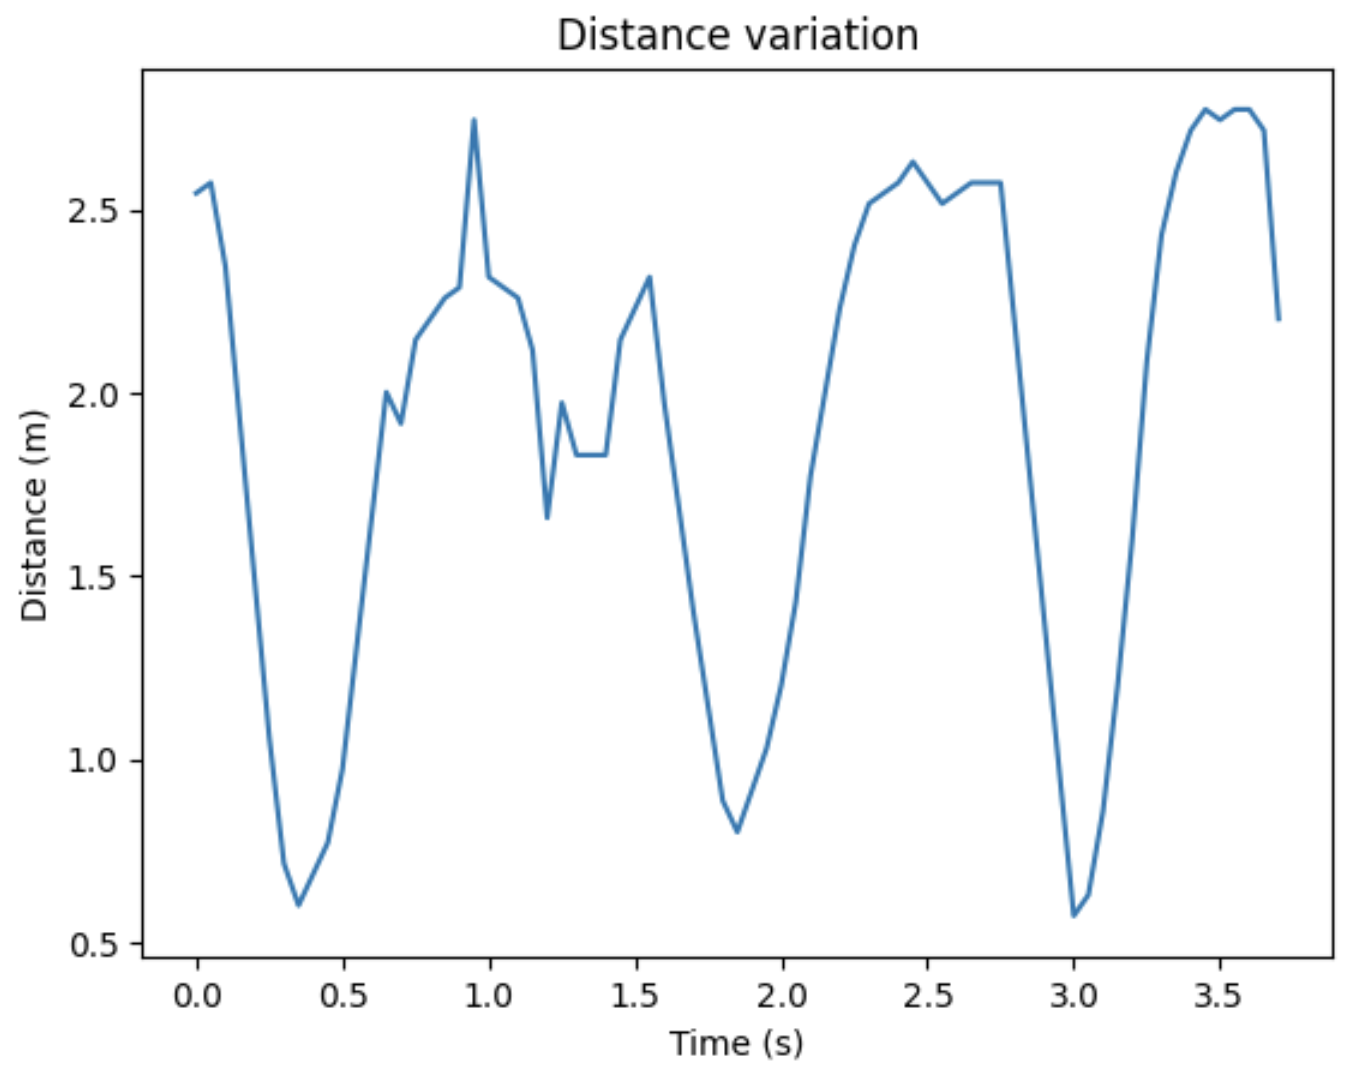
\includegraphics[width=\textwidth]{images/fast-time.png}
    \end{subfigure}
    \hfill
    \begin{subfigure}[b]{0.48\textwidth}
        \centering
        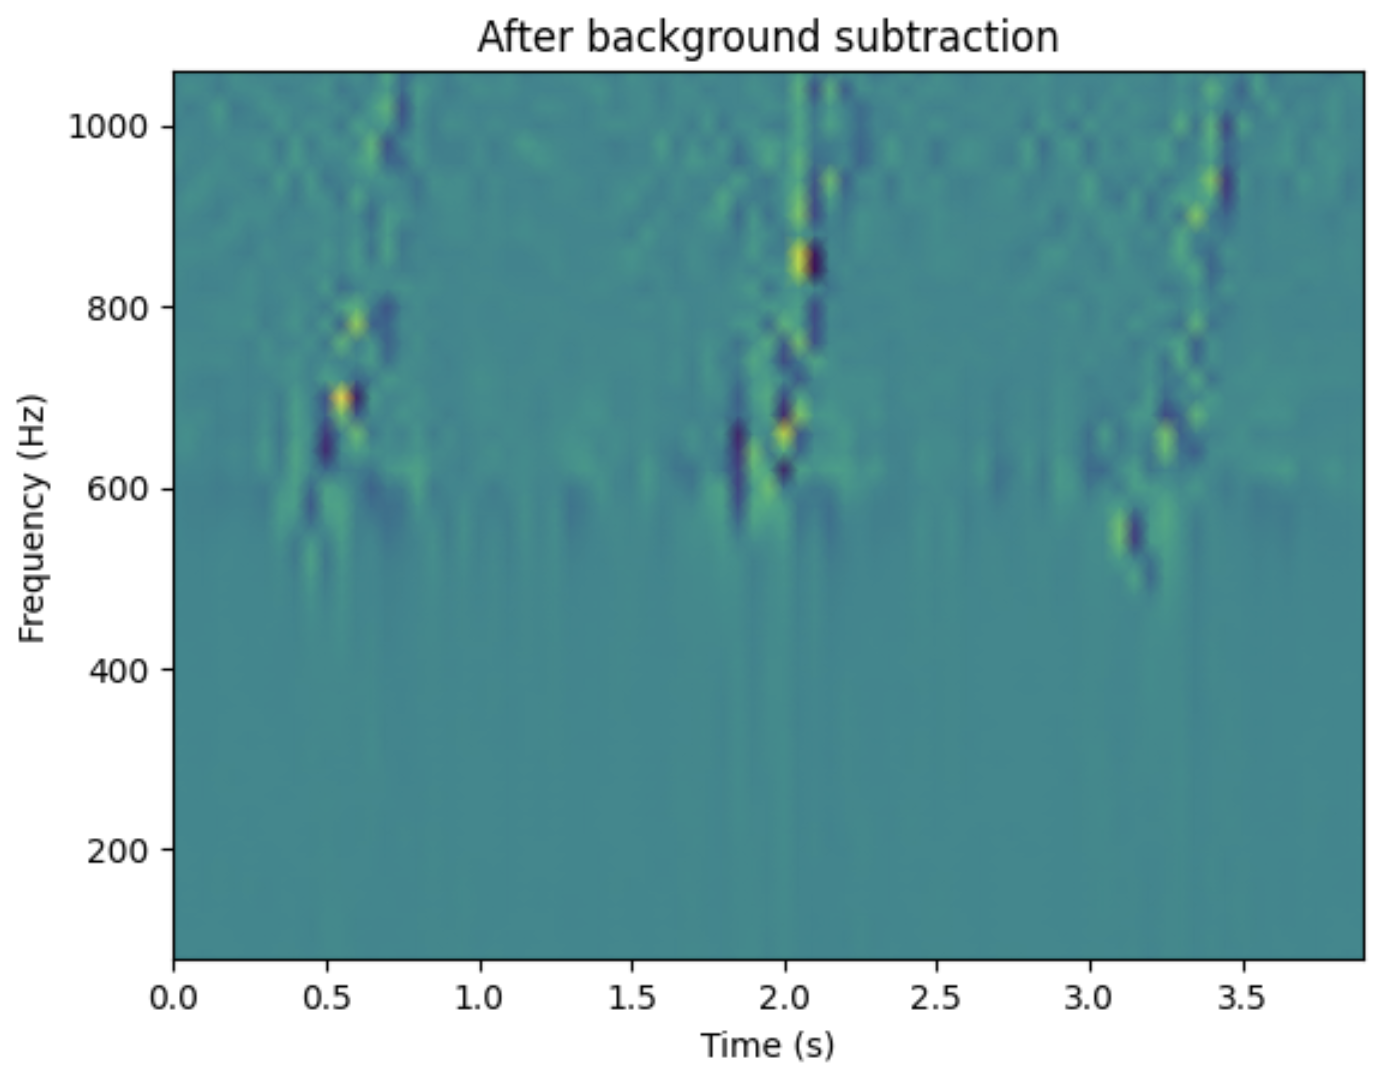
\includegraphics[width=\textwidth]{images/fast-freq.png}
    \end{subfigure}
    \caption{Fast experiment. Time and Frequency plots.}
\end{figure}


\section{Time Spent} 

Time spent:

% list of items:
\begin{itemize}
  \item Section 1: = 3 hour
  \item Section 2: = 3 hour
  \item Report: = 1 hour
\end{itemize}


\end{document}

